% !TEX root = ./ECEN-629 - Homework 2 - Brody Jordan.tex

\documentclass[11pt]{article}

\usepackage[
    assignmentDueDate={September 30, 2025 at 11:59 pm}
]{C:/Users/bljor/Sync/Courses/assignment}

\usetikzlibrary{arrows, intersections, calc}
\newcommand{\drawpolar}[4]{\draw[thick] (#1,#2) -- ({#1+#3**cos(#4)}, {#2+#3**sin(#4)});}
\usepackage{physics}
\tikzset{>=latex}
\usetikzlibrary{intersections}
\usetikzlibrary{patterns}


\begin{document}
\makeAssignmentTitle

% ——————— PROBLEM 1 —————— %
\begin{homeworkProblem}
    Suppose $f : \R \rightarrow \R$ is concave, and $a, b \in \dom f$ with $a < b$.
    \begin{enumerate}[label=(\alph*), topsep=5pt, itemsep=5pt]
        \item Prove the following inequality:
              \[
                  \frac{f(x) - f(a)}{x - a} \geq \frac{f(b) - f(a)}{b - a} \geq \frac{f(b) - f(x)}{b - x}.
              \]
              for any $x \in (a, b)$.
        \item For $f = -x^2 + 2x + 5$, $a = 0$, and $b = 3$, draw a sketch to illustrate the inequalities above.
    \end{enumerate} \vspace{1\baselineskip}

    \solution

    With $x \in (a, b)$, we can write $x = \theta a + (1-\theta) b$ which gives $\theta = (x-b)/(a-b)$ for $a\neq b$.
    \begin{align*}
        f(\theta a + (1-\theta) b) & \geq \theta f(a) + (1-\theta) f(b)                             \\
        f(x)                       & \geq \frac{x-b}{a-b} f(a) + \frac{a-x}{a-b} f(b)               \\
        f(x) - f(a)                & \geq \left(\frac{b-x}{b-a}-1\right) f(a) + \frac{a-x}{a-b}f(b) \\
        f(x) - f(a)                & \geq \frac{x - a}{b - a} f(b) - \frac{x - a}{b - a} f(a)       \\
        \frac{f(x) - f(a)}{x - a}  & \geq \frac{f(b) - f(a)}{b - a}
    \end{align*}
    And similarly for the right two inequality terms. \\

    \textbf{Part (b):} For $f(x) = -x^2 + 2x + 5$, $a = 0$, and $b = 3$ and $x = 1$:
    \begin{figure}[hbpt!]
        \vspace{\baselineskip}
        \centering
        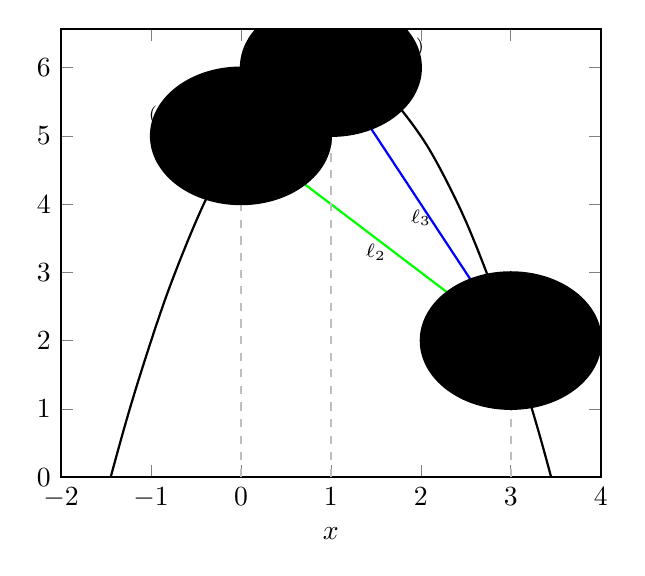
\begin{tikzpicture}
            \begin{axis}[
                    thick,
                    xlabel={$x$},
                    ymin=0,
                    xmin=-2, xmax=4,
                    ytick={0,1,2,3,4,5,6}
                    % xaxis tick for a and b
                ]
                \addplot[black, smooth] {-x^2 + 2*x + 5};
                \draw[red] (axis cs:0,5) -- (axis cs:1,6);
                \draw[green] (axis cs:0,5) -- (axis cs:3,2);
                \draw[blue] (axis cs:1,6) -- (axis cs:3,2);

                % add labels \ell_1, \ell_2, and \ell_3
                \node at (axis cs:0.5,5.25) {\scriptsize$\ell_1$};
                \node at (axis cs:2,3.8) {\scriptsize$\ell_3$};
                \node at (axis cs:1.5,3.3) {\scriptsize$\ell_2$};

                % dashed line for a, b, and x
                \draw[dashed, gray!50] (axis cs:0,0) -- (axis cs:0,5);
                \draw[dashed, gray!50] (axis cs:3,0) -- (axis cs:3,2);
                \draw[dashed, gray!50] (axis cs:1,0) -- (axis cs:1,6);

                % points and labels for (a, f(a)), (b, f(b)), and (x, f(x))
                \draw[fill] (axis cs:0,5) circle [radius=1] node [above left] {\scriptsize$(a, f(a))$};
                \draw[fill] (axis cs:3,2) circle [radius=1] node [below right] {\scriptsize$(b, f(b))$};
                \draw[fill] (axis cs:1,6) circle [radius=1] node [above right] {\scriptsize$(x, f(x))$};
            \end{axis}
        \end{tikzpicture}
    \end{figure}


\end{homeworkProblem}

\pagebreak

% ——————— PROBLEM 2 —————— %
\begin{homeworkProblem}
    Show that the maximum of a convex function $f$ over the polyhedron $\mathcal{P} = \conv \{v_1, v_2, \dots, v_k\}$ is
    achieved at one of the vertices, that is
    \[
        \sup_{x \in \mathcal{P}} f(x) = \max_{i=1,2,\dots,k} f(v_i).
    \]
    In particular, let $f(x)=x_1^2+2 x_1 x_2+3 x_2^2$, and let $v_1=(1,1)^T$, $v_2=(1,-1)^T$, $v_3=(-1, 1)^T$, and $v_4=(-1,-1)^T$. Compute its maximum over the polyhedron. \\

    \solution

    From the text, we know that the convex hull of a set is the set of all convex combinations
    of points in that set. We can express $\mathcal{P}$ as
    \[
        \mathcal{P} = \left\{\theta_1 v_1 + \dots + \theta_k v_k \mid \theta_1 + \dots + \theta_k = 1, \theta_i \geq 0, i = 1, \dots, k\right\}.
    \]
    Thus, since any point $x \in \mathcal{P}$ can be expressed as a convex combination of the vertices $v_1, v_2, \dots, v_k$, we have
    \[
        f(x) = f\left(\sum_{i=1}^{k} \theta_i v_i\right)
    \]
    Since $f$ is a convex function, by Jensen's inequality,
    \[
        f\left(\sum_{i=1}^{k} \theta_i v_i\right) \leq \sum_{i=1}^{k} \theta_i f(v_i)
    \]
    This value is maximized when $f(v_i)$ is maximized. Thus,
    \[
        f(x) \leq \max_{v_i\in\mathcal{P}} f(v_i) \sum_{i=1}^{k} \theta_i \implies \sup_{x \in \mathcal{P}} f(x) = \max_{i=1,2,\dots,k} f(v_i).
    \]

    Now we have $f(x)=x_1^2+2 x_1 x_2+3 x_2^2$, and $v_1=(1,1)^T$, $v_2=(1,-1)^T$, $v_3=(-1, 1)^T$, and $v_4=(-1,-1)^T$. We can compute
    \begin{align*}
        f(v_1) & = f((1,1)^T) = 6, \quad f(v_2) = f((1,-1)^T) = 2,    \\
        f(v_3) & = f((-1, 1)^T) = 2, \quad f(v_4) = f((-1,-1)^T) = 6.
    \end{align*}
    Thus, the maximum over the polyhedron is $6$.
\end{homeworkProblem}

\pagebreak

% ——————— PROBLEM 3 —————— %
\begin{homeworkProblem}
    Suppose
    \[
        f(x) = h(g_1(x),g_2(x)),
    \]
    where $g_1(x) = \norm{x}_2^2$, $g_2(x) = \norm{x}_1$, and $h(u, v) = \log(e^u + e^v)$.
    \begin{enumerate}[label=(\alph*), topsep=5pt, itemsep=2.5pt]
        \item Show $f(x)$ is convex by applying the correct composition rule.
        \item Give another $h$ that keeps $f$ convex but is non-logarithmic, and explain why.
    \end{enumerate} \vspace{1\baselineskip}

    \solution

    \textbf{Part (a):} $h$ presents a log-sum-exp form, which is convex when both $g_1$ and $g_2$ are convex.
    Since both $g_1$ and $g_2$ are convex (all norms are convex), we can conclude that $f(x)$ is convex. \\

    \textbf{Part (b):} Very many functions work here. Simply $h(u, v) = u + v$ works, as the sum of two convex functions is also convex.

\end{homeworkProblem}

\pagebreak

% ——————— PROBLEM 4 —————— %
\begin{homeworkProblem}
    Let $f_1, f_2, \dots, f_m$ be convex function on $\R[n]$. Define
    \[
        f(x)=\inf \left\{f_1\left(x_1\right)+f_2\left(x_2\right)+\ldots+f_m\left(x_m\right) \mid x_i \in \R[n], x_1+x_2+\ldots+x_m=x\right\} .
    \]
    Show $f(x)$ is convex on $\R[n]$. \\

    \solution

    Since each $f_1, f_2, \dots, f_m$ is convex, we have
    \[
        f_i \left(\theta x_i + (1-\theta) y_i\right) \leq \theta f_i(x_i) + (1-\theta) f_i(y_i)
    \]
    Thus, for our main function,
    \[
        f(\theta x + (1-\theta) y) \leq \sum_{i=1}^{m} \left(\theta f_i(x_i) + (1-\theta) f_i(y_i)\right)
    \]
    And taking the infimum over all $x_i$ and $y_i$ preserves the inequality, so
    \[
        f(x) = \inf \left\{f_1\left(x_1\right)+f_2\left(x_2\right)+\ldots+f_m\left(x_m\right) \mid x_i \in \R[n], x_1+x_2+\ldots+x_m=x\right\}
    \]
    is convex.

\end{homeworkProblem}

\pagebreak

% ——————— PROBLEM 5 —————— %
\begin{homeworkProblem}
    The $r$-separation function $\Delta_r(x)$ of the vector $x \in \R[n]$, where $r \leq n$, is defined as the difference between the sum
    of the $r$ largest components of the vector $x$ and the sum of the $r$ smallest components.
    \begin{enumerate}[label=(\alph*), topsep=5pt, itemsep=2.5pt]
        \item Is the function $\Delta_r(x)$ convex? Prove your answer.
        \item Let $r = 1$ and $n = 2$. Sketch the function $\Delta_1(x)$ in the positive quadrant.
    \end{enumerate} \vspace{1\baselineskip}

    \solution

    \textbf{Part (a):} The function $\Delta_r(x)$ written out:
    \[
        \Delta_r(x) = \sum_{r \text{ largest}} x_i - \sum_{r \text{ smallest}} x_i
    \]

    We know from the notes that the sum of $r$ largest components of $x \in \R[n]$ is convex. It is obvious when presented as
    \[
        f(x) = \max \{x_{i1} + x_{i2} + \ldots + x_{ir} \mid 1 \leq i_1 < i_2 < \ldots < i_r \leq n\}
    \]
    and the $r$ smallest components is concave, but the minus sign makes it convex. \\

    Since we are adding $\Delta_r(x) = f(x) + (-g(x))$, where both $f$ and $-g$ are convex, we can conclude that $\Delta_r(x)$ is convex, by the convex summation property. \\

    \textbf{Part (b):} For $r = 1$ and $n = 2$,

    \begin{figure}[hbpt!]
        \centering
        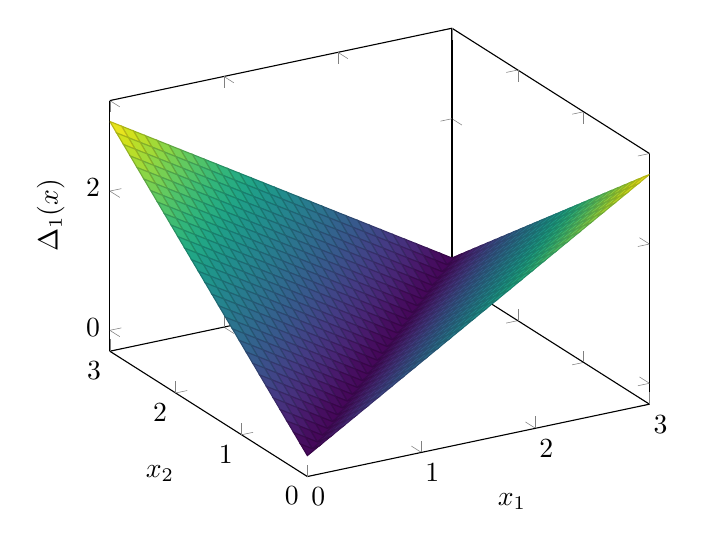
\begin{tikzpicture}
            \begin{axis}[
                    view={-30}{30},
                    domain=0:3,
                    y domain=0:3,
                    samples=30,
                    xlabel={$x_1$},
                    ylabel={$x_2$},
                    zlabel={$\Delta_1(x)$},
                    colormap/viridis,
                    mesh/ordering=y varies
                ]
                \addplot3[surf] {abs(x-y)};
            \end{axis}
        \end{tikzpicture}
    \end{figure}

\end{homeworkProblem}

\pagebreak

% ——————— PROBLEM 6 —————— %
\begin{homeworkProblem}
    Suppose $f : \R[m] \rightarrow \R$ is convex, and $A \in \R[m\times n]$, $b \in \R[m]$, $c \in \R[n]$, and $d \in \R$. Show that the function
    that $g : \R[n] \rightarrow \R$ is convex, where
    \[
        g(x) = (c^T x + d) f\left(\frac{Ax + b}{c^T x + d}\right), \quad \dom g = \{x \mid c^T x + d > 0\}.
    \]
    Provide a clear argument which rules you are applying, and the exact manner of function composition. \\

    \solution

    We have the perspective of some function $f: \R[n] \to \R$ defined as $g: \R[n] \times \R \to \R$,
    \[
        g(x, t) = t f(x/t), \quad \dom g = \{(x, t) \mid x/t \in \dom f, t > 0\}.
    \]
    $g$ is convex if $f$ is convex. \\

    Here, $x = Ax + b$ and $t = c^T x + d$, which is affine. Since convexity is preserved during composition with affine functions, $g$ is also convex.


\end{homeworkProblem}

\pagebreak

% ——————— PROBLEM 7 —————— %
\begin{homeworkProblem}
    A vector-valued function $f : \R[n] \rightarrow \R[n]$ is called monotone if $\left< f(x) - f(y), x - y\right> \geq 0$. Show that
    the gradient of a convex function is monotone. \\

    \solution

    If the gradient of a convex function is monotone, then
    \[
        \left< \nabla f(x) - \nabla f(y), x - y\right> \geq 0
    \]

    By the 1st-order condition,
    \[
        f(y) \geq f(x) + \nabla f(x)^T (y - x) = f(x) + \left< \nabla f(x), y - x \right>
    \]
    and
    \[
        f(x) \geq f(y) + \nabla f(y)^T (x - y) = f(y) + \left< \nabla f(y), x - y \right>
    \]
    Adding these two, we get
    \begin{align*}
        f(x) + f(y) & \geq f(x) + f(y) + \left< \nabla f(x), y - x \right> + \left< \nabla f(y), x - y \right> \\
        0           & \geq \left< \nabla f(x), y - x \right> + \left< \nabla f(y), x - y \right>               \\
                    & = \left< \nabla f(x) - \nabla f(y), y - x \right>                                        \\
                    & = -\left< \nabla f(x) - \nabla f(y), x - y \right>
    \end{align*}
    Thus,
    \[
        \left< \nabla f(x) - \nabla f(y), x - y \right> \geq 0
    \]
    proving that the gradient of a convex function is monotone.

\end{homeworkProblem}

\pagebreak

% ——————— PROBLEM 8 —————— %
\begin{homeworkProblem}
    The proximal operator of a function $f : \R[n] \rightarrow \R \cup \{\infty\}$ is defined by
    \[
        \prox_{\lambda f}(v) = \argmin[x] \left(f(x) + \frac{1}{2\lambda} \norm{x - v}_2^2\right).
    \]
    \begin{enumerate}[label=(\alph*), topsep=5pt, itemsep=2.5pt]
        \item Is the proximal operator a convex function?
        \item Derive the proximal operator for $f(x) = \norm{x}_1$.
        \item Solve explicitly for $v = (3, -2, 0.5)^T$ and $\lambda = 1$ when $f(x) = \norm{x}_1$.
    \end{enumerate} \vspace{1\baselineskip}

    \solution

    \textbf{Part (a):} Since $\nabla^2 p \not{\succeq} 0$, the proximal operator is not convex. \\

    \textbf{Part (b):} Now $f(x) = \norm{x}_1$. Thus, we have
    \begin{align*}
        \prox_{\lambda f}(v) & = \argmin[x] \left(\norm{x}_1 + \frac{1}{2\lambda} \norm{x - v}_2^2\right) \\
                             & = 1/\lambda (x-v)
    \end{align*}


    \textbf{Part (c):} Here $v = (3, -2, 0.5)^T$, $\lambda = 1$, and $f(x) = \norm{x}_1$. I'll plot each dimension of the function to see its minimum.

    % Plotting each dimension of the function (3 different lines)
    % First line is |x| + 1/2 (x-3)^2
    % Second line is |x| + 1/2 (x+2)^2
    % Third line is |x| + 1/2 (x-0.5)^2
    \begin{figure}[hbpt!]
        \centering
        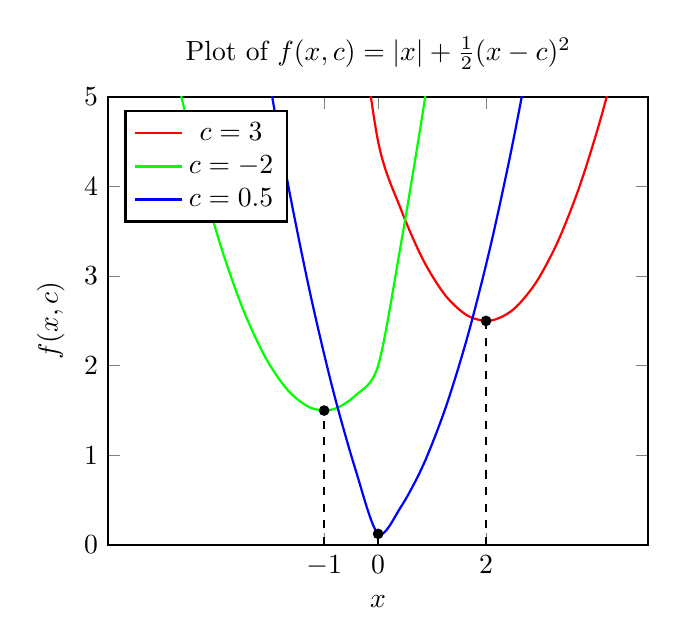
\begin{tikzpicture}
            \begin{axis}[
                    thick,
                    xlabel={$x$},
                    ylabel={$f(x, c)$},
                    ymin=0, ymax=5,
                    xmin=-5, xmax=5,
                    title={Plot of $f(x, c) = |x| + \frac{1}{2}(x-c)^2$},
                    legend pos=north west,
                    xtick={-1,0,2},
                ]
                % Plot 1: |x| + 1/2 * (x-3)^2
                \addplot[red, smooth] {abs(x) + 0.5*(x-3)^2};
                \addlegendentry{$c=3$};

                % Plot 2: |x| + 1/2 * (x+2)^2
                \addplot[green, smooth] {abs(x) + 0.5*(x+2)^2};
                \addlegendentry{$c=-2$};

                % Plot 3: |x| + 1/2 * (x-0.5)^2
                \addplot[blue, smooth] {abs(x) + 0.5*(x-0.5)^2};
                \addlegendentry{$c=0.5$};

                % add point and dotted lines for minimums
                \addplot[only marks, mark=*, mark size=1.5pt] coordinates {(2,2.5) (-1,3/2) (0,0.125)};
                \draw[dashed] (axis cs:2,0) -- (axis cs:2,2.5);
                \draw[dashed] (axis cs:-1,0) -- (axis cs:-1,3/2);
                \draw[dashed] (axis cs:0,0) -- (axis cs:0,0.125);

            \end{axis}
        \end{tikzpicture}
    \end{figure}

    From the graph, we can see that the minimums are at $x = 2$, $x = -1$, and $x = 0$.

\end{homeworkProblem}

\pagebreak

% ——————— PROBLEM 9 —————— %
\begin{homeworkProblem}
    Given a norm $\norm{\, \cdot \, }$ on $\R[n]$, the dual norm is defined as
    \[
        \norm{y}_* = \sup_{\norm{x} \leq 1} y^T x.
    \]
    \begin{enumerate}[label=(\alph*), topsep=5pt, itemsep=2.5pt]
        \item Show that $\norm{\, \cdot \, }_*$ is indeed a norm.
        \item Compute the dual norm of $\norm{x}_1$ and $\norm{x}_\infty$.
        \item For $x = (1, 2)^T$, compute $\norm{x}_2^*$.
    \end{enumerate} \vspace{1\baselineskip}

    \solution

    \textbf{Part (a):} To be a norm it must satisfy the triangle inequality
    \[
        \norm{y_1 + y_2}_* = \norm{y_1}_* + \norm{y_2}_* \quad\to\quad \sup_{\norm{x} \leq 1} (y_1 + y_2)^T x \leq \sup_{\norm{x} \leq 1} y_1^T x + \sup_{\norm{x} \leq 1} y_2^T x
    \]
    which holds by the properties of supremum. \\

    It must also satisfy absolute homogeneity
    \[
        \norm{s y}_* = |s| \norm{y}_* \quad\to\quad \sup_{\norm{x} \leq 1} (s y)^T x = |s| \sup_{\norm{x} \leq 1} y^T x
    \]
    this condition also holds since $\sup(s y) = s \sup(y)$. \\

    Finally, non-negativity, which is also satisfied by the norm definition. \\

    \textbf{Part (b):} For $\norm{x}_1$, the dual norm is simply the $l_\infty$ norm and vice versa. \\

    \textbf{Part (c):} For $x = (1, 2)^T$, $\norm{x}_2^* = \norm{x}_2 = \sqrt{1^2 + 2^2} = \sqrt{5}$.


\end{homeworkProblem}
\end{document}